\begin{figure}
    \centering
    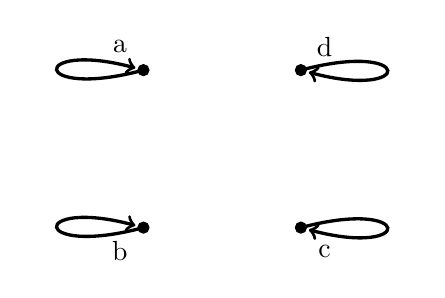
\begin{tikzpicture}

%% vertices
\draw[fill=black] (0,2) circle (2pt);   %% a
\draw[fill=black] (0,0) circle (2pt);   %% b
\draw[fill=black] (2,0) circle (2pt);   %% c
\draw[fill=black] (2,2) circle (2pt);   %% d


%% vertex labels
\node at (-0.3,2.3) {a};
\node at (-0.3,-0.3) {b};
\node at (2.3,-0.3) {c};
\node at (2.3,2.3) {d};


%%% edges
\draw[-{>[sep=3pt]}, very thick] (0,2) to [loop left, min distance=1.5cm] (0,2);     %% aa
\draw[-{>[sep=3pt]}, very thick] (0,0) to [loop left, min distance=1.5cm] (0,0);     %% bb
\draw[-{>[sep=3pt]}, very thick] (2,0) to [loop right, min distance=1.5cm] (2,0);     %% cc
\draw[-{>[sep=3pt]}, very thick] (2,2) to [loop right, min distance=1.5cm] (2,2);     %% dd
    \end{tikzpicture}
    \label{q4-a}
    \caption{Reflexive relation}
\end{figure}